% ==============================================================
% 세종과학예술영재학교 졸업논문 양식                                                                            
% ==============================================================
% XeLaTeX로 조판하여야 합니다!
% 졸업논문 양식 사용방법에 대해 더 알고 싶거나 궁금한 사항은 세종과학예술영재학교 3기 신주형, 강태원 학생에게 질문해 주시기 바랍니다. 
% 교내 졸업논문을 TeX 양식으로 사용할 수 있도록 도와주신 권현우님께 진심으로 감사 인사를 전합니다.
% ==============================================================

\documentclass{thesis-SJ}

\title[English title]{논문제목}
% 논문 제목 [영어제목]{한글제목} 을 기재합니다.
\authorone[洪日東]{홍일동}{Hong, Il Dong}{3101}
\authortwo[洪理東]{홍이동}{Hong, Lee Dong}{3202}
%\authorthree[洪森東]{홍삼동}{Hong, Lee Dong}{3303}
%\authorfour[洪瀉東]{홍사동}{Hong, Sa Dong}{3404}
% 저자정보 [한자성명]{성명}{영어성명}{학번}을 기재합니다.

\advisor{홍길순}{Gilsoon Hong}
\teacher{홍길남}{Gilnam Hong}
% Thesis Advisor와 지도교사 성명을 기재합니다.

\referee[1]{이순신}
\referee[2]{권율}
% 심사위원 이름을 기재합니다.

\date{2019년 5월 8일}{May 8th, 2019}
% 학위청구논문 심사 통과일을 기재합니다.

\usepackage{graphicx}

\begin{document}
	\newpage
	\tableofcontents
	\listoftables
	\listoffigures
	
	%%% 영문 초록 %%%
	
	\newpage
	\EnglishAbstract
	% Abstract(초록) 을 여기서부터 영문으로 작성합니다.
	% Abstract의 내용은 영문 1000자 미만으로 작성합니다.
	Lorem Ipsum is simply dummy text of the printing and typesetting industry. Lorem Ipsum has been the industry's standard dummy text ever since the 1500s, when an unknown printer took a galley of type and scrambled it to make a type specimen book. It has survived not only five centuries, but also the leap into electronic typesetting, remaining essentially unchanged. It was popularised in the 1960s with the release of Letraset sheets containing Lorem Ipsum passages, and more recently with desktop publishing software like Aldus PageMaker including versions of Lorem Ipsum.

	\EnglishKeywords{English keywords}
	
	%%% 한글 초록 %%%
	
	\KoreanAbstract
	% Abstract(초록) 을 여기서부터 한글로 작성합니다.
	% Abstract의 내용은 국문 600자 미만으로 작성합니다.
	하수(河水)는 두 산 틈에서 나와 돌과 부딪쳐 싸우며, 그 놀란 파도와 성난 물머리와 우는 여울과 노한 물결과 슬픈 곡조와 원망하는 소리가 굽이쳐 돌면서, 우는 듯, 소리치는 듯, 바쁘게 호령하는 듯, 항상 장성을 깨뜨릴 형세가 있어, 전차(戰車) 만승(萬乘)과 전기(戰騎) 만대(萬隊)나 전포(戰砲) 만가(萬架)와 전고(戰鼓) 만좌(滿座)로써는 그 무너뜨리고 내뿜는 소리를 족히 형용할 수 없을 것이다. 모래 위에 큰 돌은 홀연히 떨어져 섰고, 강 언덕에 버드나무는 어둡고 컴컴하여 물지킴과 하수 귀신이 다투어 나와서 사람을 놀리는 듯한데, 좌우의 교리(蛟 )가 붙들려고 애쓰는 듯싶었다.
	
	\KoreanKeywords{Korean keywords}
	
	
	\mainpartstart
	\newpage
	
<<<<<<< HEAD
	% ===================== 여기서부터 논문을 작성하시면 됩니다. ===================== 
	\chapter{이론적 배경} 
	\section{다람쥐 헌 쳇바퀴에 타고파}
	\subsection{이론 1}
	선거에 관한 경비는 법률이 정하는 경우를 제외하고는 정당 또는 후보자에게 부담시킬 수 없다. 공개하지 아니한 회의내용의 공표에 관하여는 법률이 정하는 바에 의한다.
=======
	% ================ 여기서부터 논문을 작성하시면 됩니다. ================ 
>>>>>>> 793112707895a5b8fd533c04a6da9e7964cb6000
	
	대한민국은 민주공화국이다. 체포·구속·압수 또는 수색을 할 때에는 적법한 절차에 따라 검사의 신청에 의하여 법관이 발부한 영장을 제시하여야 한다. 다만, 현행범인인 경우와 장기 3년 이상의 형에 해당하는 죄를 범하고 도피 또는 증거인멸의 염려가 있을 때에는 사후에 영장을 청구할 수 있다.
	
	국군은 국가의 안전보장과 국토방위의 신성한 의무를 수행함을 사명으로 하며, 그 정치적 중립성은 준수된다. 국가안전보장회의의 조직·직무범위 기타 필요한 사항은 법률로 정한다.
	
	누구든지 병역의무의 이행으로 인하여 불이익한 처우를 받지 아니한다. 감사원의 조직·직무범위·감사위원의 자격·감사대상공무원의 범위 기타 필요한 사항은 법률로 정한다.
	
	헌법재판소 재판관은 탄핵 또는 금고 이상의 형의 선고에 의하지 아니하고는 파면되지 아니한다. 공무원인 근로자는 법률이 정하는 자에 한하여 단결권·단체교섭권 및 단체행동권을 가진다.
	
	군사법원의 조직·권한 및 재판관의 자격은 법률로 정한다. 대한민국의 국민이 되는 요건은 법률로 정한다. 헌법재판소에서 법률의 위헌결정, 탄핵의 결정, 정당해산의 결정 또는 헌법소원에 관한 인용결정을 할 때에는 재판관 6인 이상의 찬성이 있어야 한다.
	
	\subsection{이론 2}
	신체장애자 및 질병·노령 기타의 사유로 생활능력이 없는 국민은 법률이 정하는 바에 의하여 국가의 보호를 받는다. 국민의 자유와 권리는 헌법에 열거되지 아니한 이유로 경시되지 아니한다. 체포·구속·압수 또는 수색을 할 때에는 적법한 절차에 따라 검사의 신청에 의하여 법관이 발부한 영장을 제시하여야 한다. 다만, 현행범인인 경우와 장기 3년 이상의 형에 해당하는 죄를 범하고 도피 또는 증거인멸의 염려가 있을 때에는 사후에 영장을 청구할 수 있다.
	
	모든 국민은 법률이 정하는 바에 의하여 공무담임권을 가진다. 모든 국민은 신속한 재판을 받을 권리를 가진다. 형사피고인은 상당한 이유가 없는 한 지체없이 공개재판을 받을 권리를 가진다. 대통령은 전시·사변 또는 이에 준하는 국가비상사태에 있어서 병력으로써 군사상의 필요에 응하거나 공공의 안녕질서를 유지할 필요가 있을 때에는 법률이 정하는 바에 의하여 계엄을 선포할 수 있다.
	
	대통령은 제1항과 제2항의 처분 또는 명령을 한 때에는 지체없이 국회에 보고하여 그 승인을 얻어야 한다. 국회는 국정을 감사하거나 특정한 국정사안에 대하여 조사할 수 있으며, 이에 필요한 서류의 제출 또는 증인의 출석과 증언이나 의견의 진술을 요구할 수 있다. 국가는 노인과 청소년의 복지향상을 위한 정책을 실시할 의무를 진다.
	
	위원은 탄핵 또는 금고 이상의 형의 선고에 의하지 아니하고는 파면되지 아니한다. 국민경제자문회의의 조직·직무범위 기타 필요한 사항은 법률로 정한다. 대통령의 임기가 만료되는 때에는 임기만료 70일 내지 40일전에 후임자를 선거한다. 광물 기타 중요한 지하자원·수산자원·수력과 경제상 이용할 수 있는 자연력은 법률이 정하는 바에 의하여 일정한 기간 그 채취·개발 또는 이용을 특허할 수 있다.
	
	국가는 농업 및 어업을 보호·육성하기 위하여 농·어촌종합개발과 그 지원등 필요한 계획을 수립·시행하여야 한다. 대한민국의 영토는 한반도와 그 부속도서로 한다. 국회는 의장 1인과 부의장 2인을 선출한다. 선거에 관한 경비는 법률이 정하는 경우를 제외하고는 정당 또는 후보자에게 부담시킬 수 없다.
	
	제안된 헌법개정안은 대통령이 20일 이상의 기간 이를 공고하여야 한다. 대통령은 법률이 정하는 바에 의하여 사면·감형 또는 복권을 명할 수 있다. 감사원의 조직·직무범위·감사위원의 자격·감사대상공무원의 범위 기타 필요한 사항은 법률로 정한다. 대통령은 조약을 체결·비준하고, 외교사절을 신임·접수 또는 파견하며, 선전포고와 강화를 한다.
	
	\begin{table}[ht]
		\centering
		\begin{tabular}{|r||c|c|}
	\hline  & 남자 & 여자 \\ \hline\hline
	$0$ & $100,000$ & $100,000$ \\ \hline
	$10$ & $95,481$ & $96,395$ \\ \hline
	$20$ & $94,590$ & $95,852$ \\ \hline
	$30$ & $92,640$ & $94,607$ \\ \hline
	$40$ & $90,285$ & $92,820$ \\ \hline
	$50$ & $85,836$ & $89,621$ \\ \hline
	$60$ & $75,257$ & $82,607$ \\ \hline
	$70$ & $53,647$ & $67,246$ \\ \hline
	\end{tabular}

		\caption{인구 조사}\label{fig:population}
	\end{table}
	국가는 모성의 보호를 위하여 노력하여야 한다. 새로운 회계연도가 개시될 때까지 예산안이 의결되지 못한 때에는 정부는 국회에서 예산안이 의결될 때까지 다음의 목적을 위한 경비는 전년도 예산에 준하여 집행할 수 있다. 대통령후보자가 1인일 때에는 그 득표수가 선거권자 총수의 3분의 1 이상이 아니면 대통령으로 당선될 수 없다.\cite{kopka1995guide}
	
	국회는 선전포고, 국군의 외국에의 파견 또는 외국군대의 대한민국 영역안에서의 주류에 대한 동의권을 가진다. 국회는 의원의 자격을 심사하며, 의원을 징계할 수 있다. 헌법개정은 국회재적의원 과반수 또는 대통령의 발의로 제안된다. 대한민국의 경제질서는 개인과 기업의 경제상의 자유와 창의를 존중함을 기본으로 한다.
	
	모든 국민은 법 앞에 평등하다. 누구든지 성별·종교 또는 사회적 신분에 의하여 정치적·경제적·사회적·문화적 생활의 모든 영역에 있어서 차별을 받지 아니한다. 헌법재판소 재판관은 탄핵 또는 금고 이상의 형의 선고에 의하지 아니하고는 파면되지 아니한다. 감사원은 원장을 포함한 5인 이상 11인 이하의 감사위원으로 구성한다.\cite{slater1994latex}
	
	모든 국민은 인간다운 생활을 할 권리를 가진다. 국회는 법률에 저촉되지 아니하는 범위안에서 의사와 내부규율에 관한 규칙을 제정할 수 있다. 국회의 회의는 공개한다. 다만, 출석의원 과반수의 찬성이 있거나 의장이 국가의 안전보장을 위하여 필요하다고 인정할 때에는 공개하지 아니할 수 있다. 비상계엄이 선포된 때에는 법률이 정하는 바에 의하여 영장제도, 언론·출판·집회·결사의 자유, 정부나 법원의 권한에 관하여 특별한 조치를 할 수 있다.
	
	
	\begin{figure}[ht]
		\centering
		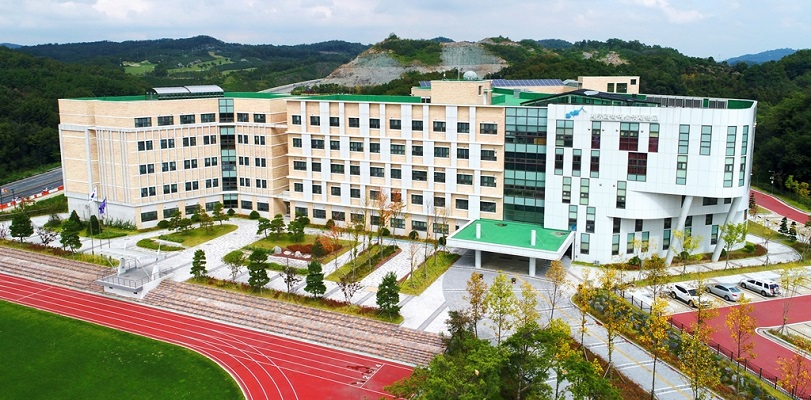
\includegraphics[width=.75\linewidth]{images/school}
		\caption{세종과학예술영재학교}
		\label{fig:school}
	\end{figure}
	
<<<<<<< HEAD
	
	\chapter{탐구 계획}
	\section{탐구 과정}
	위원은 탄핵 또는 금고 이상의 형의 선고에 의하지 아니하고는 파면되지 아니한다.
	
	군사법원의 조직·권한 및 재판관의 자격은 법률로 정한다. 사회적 특수계급의 제도는 인정되지 아니하며, 어떠한 형태로도 이를 창설할 수 없다.
	
	국회의 회의는 공개한다. 다만, 출석의원 과반수의 찬성이 있거나 의장이 국가의 안전보장을 위하여 필요하다고 인정할 때에는 공개하지 아니할 수 있다.
	
	모든 국민은 통신의 비밀을 침해받지 아니한다. 탄핵결정은 공직으로부터 파면함에 그친다. 그러나, 이에 의하여 민사상이나 형사상의 책임이 면제되지는 아니한다.
	
	근로조건의 기준은 인간의 존엄성을 보장하도록 법률로 정한다.\cite{lamport1994latex}
	
	\begin{figure}[ht]
		\centering
		
\includegraphics[width=.75\linewidth]{images/minttrash}
		\caption{음식물 쓰레기}
		\label{fig:minttrash}
	\end{figure}
%%% 참고 문헌 %%%
\makebibliography
=======
	% ============================================================
	
% ================ 여기서부터 참고 문헌을 작성하시면 됩니다. =================
\begin{thebibliography}{10}
	\bibitem{1}
	Chang, I. (2010). “Biopolymer treated Korean Residual Soil: Geotechnical behavior and Applications”,  Ph.D. Thesis, Korea Advanced Institute of Science and Technology, Daejeon, Republic of Korea, 320 pages.
	
	% 단행본(Book)의 예시
	\bibitem{2}
	Grim, R. (1962). Applied clay mineralogy, McGraw-Hill, NewYork, 160 pages.
	
	% 특허(Patents)의 경우 예시
	\bibitem{3}
	J.L. Lee et al. (1998). "GaAs Power Semiconductor Device Operating at a Low Voltage and Method for Fabricating the Same", US Patent 5, 760, 418, to ETRI, Patent and Trademark Office, Washington D.C., 1998.
	
	% 학회논문(Conference proceeding)의 경우 예시
	\bibitem{4}
	Mgangira, M.B. (2009). "Evaluation of the effects of enzyme-based liquid chemical stabilizers on subgrade soils." 28th Annual Southern African Transport Conference (SATC) 2009, Pretoria, South Africa, pp. 192-199.
	
	% 저널아티클(Periodicals)의 경우 예시
	\bibitem{5}
	Noborio, K., McInnes, K. J., and Heilman, J. L. (1996). "Measurements of Soil Water Content, Heat Capacity, and Thermal Conductivity With A Single Tdr Probe1."  Soil Science, 161(1), pp. 22-28.
	
\end{thebibliography}
% ==============================================================
	
>>>>>>> 793112707895a5b8fd533c04a6da9e7964cb6000
\end{document}
